\documentclass{article}

\usepackage[inline]{enumitem}
\usepackage{amsmath}
\usepackage{graphicx}

\newcommand{\ds}{\displaystyle}

\begin{document}

\noindent{}\rule{\textwidth}{0.4pt}
\begin{center}
	Universidade Federal da Grande Dourados\\
	An\'alise Num\'erica --- Lista 4 \\
	Engenharia Mec\^anica --- 2016.2 \\
	Prof.\ Adriano Barbosa
\end{center}
\noindent{}\rule{\textwidth}{0.4pt}

\begin{enumerate}
	\item Calcule o polin\^omio interpolador de Lagrange de grau no m\'aximo 1 e 2
		para as fun\c{c}\~oes abaixo e $x_0=0$, $x_1=0.6$ e $x_2=0.9$. Utilize o
		polin\^omio para aproximar o valor de $f(0.45)$ e calcule o erro
		absoluto.
		\begin{enumerate}
			\item $f(x) = \cos{x}$
			\item $f(x) = \sqrt{1+x}$
			\item $f(x) = \ln{(x+1)}$
			\item $f(x) = \tan{x}$
		\end{enumerate}
	
	\item Use o Teorema do erro para as aproxima\c{c}\~oes do exerc\'{\i}cio anterior.
		Compare com o erro absoluto calculado.

	\item Use o polin\^omio interpolador de Lagrange de grau 1, 2 e 3
		para aproximar cada um dos valores abaixo:
		\begin{enumerate}
			\item $f(8.4)$, onde $f(8.1) = 16.94410$, $f(8.3) = 17.56492$,
				$f(8.6) = 18.50515$, $f(8.7) = 18.82091$
			\item $f\left(\ds-\frac{1}{3}\right)$, onde $f(-0.75) =
				-0.07181250$, $f(-0.5)=-0.02475000$, $f(-0.25) = 0.33493750$,
				$f(0)=1.10100000$
			\item $f(0.25)$, onde $f(0.1) = -0.62049958$, $f(0.2) =
				-0.28398668$, $f(0.3) = 0.00660095$, $f(0.4) = 0.24842440$
			\item $f(0.9)$, onde $f(0.6) = -0.17694460$, $f(0.7) = 0.01375227$,
				$f(0.8) = 0.22363362$, $f(1.0) =0.65809197$
		\end{enumerate}

	\item Os valores do exerc\'{\i}cio anterior s\~ao das fun\c{c}\~oes abaixo. Use a Teorema do erro para calcular o limitante do erro e compare com os resultados obtidos para os polin\^omios de grau 1 e 2.
		\begin{enumerate}
			\item $f(x) = x \ln{x}$
			\item $f(x) = x^3 + 4.001x^2 + 4.002x + 1.101$
			\item $f(x) = x\cos{x} -2x^2 + 3x -1$
			\item $f(x) = \sin{(e^x-2)}$
		\end{enumerate}
		
	\item Seja $P_3(x)$ o polin\^omio interpolador para o dado $(0,0)$, $(0.5,
		y)$, $(1,3)$ e $(2,2)$. O coeficiante de $x^3$ em $P_3(x)$ \'e $6$.
		Calcule o valor de $y$.

	\item A tabela abaixo apresenta a popula\c{c}\~ao dos Estados Unidos entre os
		anos $1950$ e $2000$.

		\begin{table}
			\begin{tabular}{c|c|c|c|c|c|c}  % chktex 44
				Ano & 1950 & 1960 & 1970 & 1980 & 1990 & 2000 \\
				\hline{}  % chktex 44
				Popula\c{c}\~ao (mil) & 151.326 & 179.323 & 203.302 &
				226.542 & 249.633 & 281.422
			\end{tabular}
		\end{table}
		
		\begin{enumerate}
			\item Use o polin\^omio interpolador de Lagrange para aproximar os
				valores da popula\c{c}\~ao nos anos $1940$, $1975$ e $2020$.
			\item Sabemos que a popula\c{c}\~ao em $1940$ era aproximadamente
				$132.165.000$. Qu\~ao precisas s\~ao as aproxima\c{c}\~oes do item
				anterior para os anos de $1975$ e $2020$. Justifique.
		\end{enumerate}

	\item O polin\^omio de Bernstein de grau $n$ para $f\in{}C[0,1]$ \'e dado por
		\[B_n(x) = \sum_{k=0}^n
			\binom{n}{k}f\left(\frac{k}{n}\right)x^k{(1-x)}^{n-k}\]
		onde $\binom{n}{k}=\frac{n!}{k!(n-k)!}$. Esses polin\^omios s\~ao
		utilizados na prova do Teorema de Aproxima\c{c}\~ao de Weierstrass, pois
		$\ds\lim_{n\rightarrow{}\infty} B_n(x) = f(x)$, para cada
		$x\in{}[0,1]$.

		Calcule $B_3(x)$ para as fun\c{c}\~oes $f(x) = x$ e $f(x) = 1$.
\end{enumerate}

Respostas:

\noindent{}1. (a) $n=1: 0.869$, erro$=0.03145$, $n=2: 0.8981$, erro$=0.00235$\\
(b) $n=1: 1.1987$, erro$=0.00546$, $n=2: 1.2034$, erro$=7.59\times{}10^{-4}$\\
(c) $n=1: 0.3525$, erro$=0.01906$, $n=2: 0.36829$, erro$=0.03273$\\
(d) $n=1: 0.5131$, erro$=0.03005$, $n=2: 0.45461$, erro$=0.02845$

\noindent{}2. (a) $0.03375$, $0.00506$ (b) $0.08438$, $0.001898$ (c) $0.03375$,
$0.01013$ \\(d) $0.06779$, $0.15104$

\noindent{}3. 
\begin{figure}[!h]
	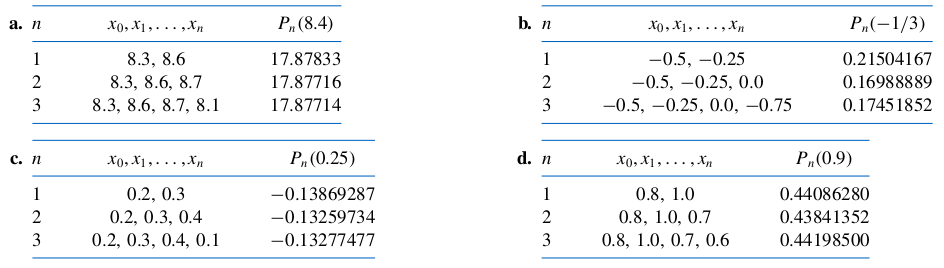
\includegraphics[width=\textwidth]{ex3.png}
\end{figure}
\newpage{}

\noindent{}4.
\begin{figure}[!h]
	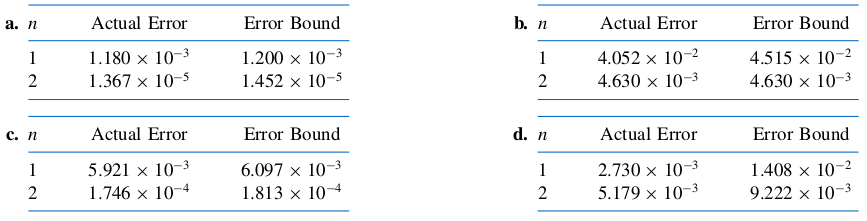
\includegraphics[width=\textwidth]{ex4.png}
\end{figure}

\noindent{}5. $y=4.25$

\noindent{}6. $102.396,953$, $215.042,718$, $513.442,968$

\noindent{}7. $B_3(x) = x$, $B_3(x) = 1$
\end{document}  % chktex 16
